\begin{table*}[t]
\small
\singlespace
\centering
\caption{Resource Usage Results}
\label{tab:resources}
\tabcolsep=0.11cm
\begin{tabular}{@{}|l|l|l|l|l|l|l|l|l|l|l|l|l|@{}}
\toprule
                    & \multicolumn{4}{l|}{\textbf{Original}}                      & \multicolumn{4}{l|}{\textbf{StitchUp}}                      & \multicolumn{4}{l|}{\textbf{DMR}}                           \\ \midrule
\textbf{Bench}      & \textit{LUT} & \textit{REG} & \textit{DSP} &\textit{Pow mW} & \textit{LUT} & \textit{REG} & \textit{DSP} &\textit{Pow mW}& \textit{LUT} & \textit{REG} & \textit{DSP} & \textit{Pow mW}   \\ \midrule
\textit{aes}        & 47230        & 28152        & 0            & 299.346        & 47539        & 28800        & 0            & 316.186        & 90467        & 53944        & 0            & -              \\ \midrule
\textit{adpcm}      & 21050        & 16752        & 168          & 133.962        & 29599        & 29484        & 178          & 156.903        & 38664        & 31077        & 348          & -              \\ \midrule
\textit{blowfish}   & 97002        & 45320        & 0            & -              & 97440        & 46039        & 0            & -              & 194598       & 88268        & 0            & -              \\ \midrule
\textit{dfadd}      & 4639         & 4310         & 0            & 50.0916        & 5562         & 5095         & 0            & 54.224         & 6394         & 5754         & 0            & 58.114         \\ \midrule
\textit{dfdiv}      & 12144        & 13157        & 30           & 100.435        & 22254        & 23449        & 60           & 145.577        & 22811        & 23904        & 60           & 147.027        \\ \midrule
\textit{dfmul}      & 3348         & 3912         & 16           & 47.024         & 4553         & 4845         & 32           & 54.128         & 5105         & 5397         & 32           & 57.521         \\ \midrule
\textit{dfsin}      & 21343        & 20347        & 71           & 137.802        & 40928        & 38116        & 136          & 222.217        & 41136        & 38321        & 142          & -              \\ \midrule
\textit{gsm}        & 11953        & 9879         & 72           & 147.006        & 22049        & 17228        & 144          & 260.730        & 22399        & 17331        & 144          & 265.949        \\ \midrule
\textit{mips}       & 8278         & 6367         & 4            & 89.326         & 15639        & 10231        & 8            & 132.409        & 14304        & 10351        & 8            & 134.316        \\ \midrule
\textit{motion}     & 52665        & 26743        & 1            & -              & 104840       & 50719        & 1            & -              & 106986       & 51199        & 2            & -              \\ \midrule
\textit{sha}        & 9117         & 9287         & 3            & -              & 9491         & 10188        & 6            & -              & 16788        & 16189        & 6            & -               \\ \bottomrule
\end{tabular}
\end{table*}

The performance of the StitchUp approach was evaluated in several ways:
firstly the error resilience and area compared to DMR for the dot product example in Listing \ref{lst:DotProduct} was
measured as the inner loop was unrolled to compute more of the computation in parallel;
secondly area and power results were found for the CHStone benchmark; and finally the error
resilience properties of CHStone benchmarks protected with StitchUp and DMR.

\subsection{Unrolling Results}
\begin{figure}[h]
\centering
\includegraphics[width=3.5in]{./graphs/dp_unrolling_res.pdf}
\caption{Data Only Errors and Caught Errors for a dot product loop unrolling with StitchUp along with \%LUT overhead against DMR}
\label{fig:dp_unrolling_res}
\end{figure}

Figure \ref{fig:dp_unrolling_res} shows how the data only errors and caught errors vary as the loop in Listing \ref{lst:DotProduct}
is unrolled.
Increasing the unroll factor reduces the control-to-data ratio as the amount of parallel (data-flow) only functional units is increased
while the number of basic blocks remains the same.
This can be observed in the graph as we increase the unroll factor the data only errors also increase while the number of caught errors
stays constant.
A similar trend can also be observed for the \%LUT overhead, where as the unroll factor increases the overhead for the DMR implementation
tends towards 100\%, while the StitchUp overhead tends towards 0\%.
This tells us that as more non-control-structure instructions are executed in parallel the overhead or
protection provided by the StitchUp replication is unaffected.

\subsection{Resource Overheads}
\renewcommand{\arraystretch}{0.8}

\begin{figure}[h]
\centering
\includegraphics[width=3.5in]{./graphs/luts_res.pdf}
\caption{Comparison of \% LUT overheads required for both StitchUp and DMR}
\label{fig:lut_res}
\end{figure}

Table \ref{tab:resources} shows the resources and power required to implement each of the CHStone benchmark circuits\footnote{with the exception of JPEG, which could not be routed onto our largest device}
with, no protection (original), StitchUp protection, and DMR protection.
Figure \ref{fig:lut_res} shows the \%LUT overhead for each circuit each protection strategy requires.
In some cases the amount of overhead control-flow and data-flow are very decoupled therefore requiring little replication, this is especially true
the encryption benchmarks (aes, blowfish, sha) where replication can be as little as \%1 of the original circuit.
While other cases the control and data flow are inseparable, such as dfsin or dfdiv, resulting in StitchUp needing the replicate
the entire circuit and performing the same as DMR.

%Power Results
\subsection{Power Results}
\begin{figure}[h]
\centering
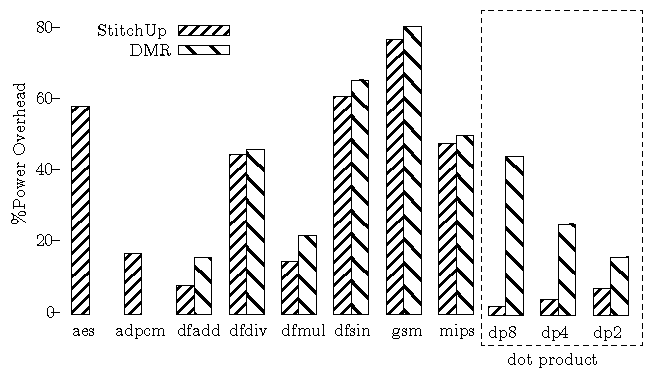
\includegraphics[width=3.5in]{./graphs/power_results.pdf}
\caption{Comparison of \% power overheads required for both StitchUp and DMR}
\label{fig:power_res}
\end{figure}

Figure \ref{fig:power_res} shows the \% power overheads for all circuits small enough to be synthesised for the ZC702 device and match the
resource overhead results, with circuits requiring more resources also requiring more power.
Along with some CHStone circuits the results for Listing \ref{lst:DotProduct} can be seen for an unroll factor 2 in dp2, unroll factor 4 in dp4,
and unroll factor 8 in dp8. 
Here we can see as the unrolling increases and the control-to-data ratio decreases the difference between the amount
of power required for full DMR and StitchUp increases.

\subsection{Fault Injection Results}

\begin{figure}[h]
\centering
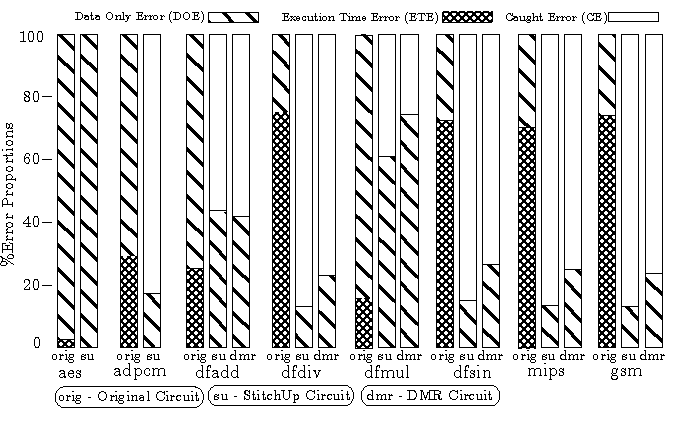
\includegraphics[width=3.5in]{./graphs/errors_res.pdf}
\caption{Error results for the CHStone benchmarks}
\label{fig:error_res}
\end{figure}

For all the benchmarks able to fit on the Zedboard device\footnote{Zedboard's have 55K Luts}
exhaustive error injection was performed, and each error was categorised into ETE, DOE, or CE.
Figure \ref{fig:error_res} shows the different proportions of these errors for each circuit, and in
all cases we can see that the ETE have been removed in the StitchUp and DMR cases.


%\begin{table*}[t]
%\small
%\singlespace
%\centering
%\caption{Fault Injection Results}
%\label{tab:faults}
%\tabcolsep=0.11cm
%\begin{tabular}{|l|l|l|l|l|l|l|l|l|l|}
%\hline
%                    & \multicolumn{3}{l|}{\textbf{Original}} & \multicolumn{3}{l|}{\textbf{StitchUp}} & \multicolumn{3}{l|}{\textbf{DMR}} \\ \hline
%\textbf{Benchmarks} & \%ETE       & \%DOE       & \%CE       & \%ETE       & \%DOE       & \%CE       & \%ETE      & \%DOE     & \%CE     \\ \hline
%\textit{aes}        &             &             &            &             &             &            &            &           &          \\ \hline
%\textit{adpcm}      &             &             &            &             &             &            &            &           &          \\ \hline
%\textit{dfadd}      &             &             &            &             &             &            &            &           &          \\ \hline
%\textit{dfdiv}      &             &             &            &             &             &            &            &           &          \\ \hline
%\textit{dfmul}      &             &             &            &             &             &            &            &           &          \\ \hline
%\textit{dfsin}      &             &             &            &             &             &            &            &           &          \\ \hline
%\textit{gsm}        &             &             &            &             &             &            &            &           &          \\ \hline
%\textit{mips}       &             &             &            &             &             &            &            &           &          \\ \hline
%\textit{sha}        &             &             &            &             &             &            &            &           &          \\ \hline
%\end{tabular}
%\end{table*}

